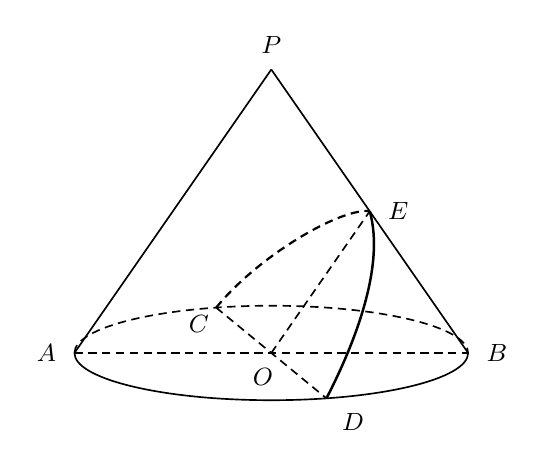
\begin{tikzpicture}[line width=0.6pt, font=\small]
\coordinate (P) at (0,3.6);
\coordinate (O) at (0,0);
\coordinate (A) at (-2.5,0);
\coordinate (B) at (2.5,0);
\coordinate (C) at (-0.7000000000,0.5760000000);
\coordinate (D) at (0.7000000000,-0.5760000000);
\coordinate (E) at (1.25,1.8);
% cone contours
\draw (P) -- (-2.5,0);
\draw (P) -- (2.5,0);
% base ellipse: back dashed, front solid
\draw (-2.5,0) arc (180:360:2.5 and 0.6);
\draw[densely dashed] (-2.5,0) arc (180:0:2.5 and 0.6);
% diameter AB dashed
\draw[densely dashed] (A) -- (B);
% interior dashed segments
\draw[densely dashed] (C) -- (O) -- (D);

\draw[densely dashed] (O) -- (E);
\draw[densely dashed,line width=.8pt] (C) .. controls (-.15,1.25) and (.9,1.85) .. (E);
% thick parabola arc E-D on side surface (schematic parabolic segment by formula)
\draw[line width=0.9pt] (E) .. controls (1.45,1.1) and (1.05,0.1) .. (D);
\node[above=2pt] at (P) {$P$};
\node[left=3pt] at (A) {$A$};
\node[right=3pt] at (B) {$B$};
\node[below=3pt,xshift=-3pt,yshift=1.0pt] at (O) {$O$};
\node[left=3pt,xshift=4pt,yshift=-6pt] at (C) {$C$};
\node[below right=2pt] at (D) {$D$};
\node[right=3pt] at (E) {$E$};
\end{tikzpicture}
